\documentclass[11pt]{amsart}
\usepackage{float}
\usepackage{amsfonts, amstext, amsmath, amsthm, amscd, amssymb, upgreek}
\usepackage{graphicx, color,  subfigure, wrapfig, overpic}
\usepackage[all,cmtip]{xy} 
\usepackage{tikz}



\textwidth 6.07in 
\textheight 8.6in 
\oddsidemargin 0.18in
\evensidemargin 0.18in
% \topmargin -0.07in
 
%%  If the following line is uncommented, we see the labels of theorems, figures, etc. in the margins.
% \usepackage[notref,notcite]{showkeys}
\setlength{\marginparwidth}{0.8in}
\let\oldmarginpar\marginpar
\renewcommand\marginpar[1]{\oldmarginpar[\raggedleft\footnotesize #1]%
{\raggedright\footnotesize #1}}

%This command stops the Math Review numbers appearing in the references! 
\AtBeginDocument{
   \def\MR#1{}
}
\newcommand{\Sp}{\rm{S}}
\newcommand{\C}{\mathbb{C}}
\newcommand{\R}{\mathbb{R}}
\newcommand{\Q}{\mathbb{Q}}
\newcommand{\Z}{\mathbb{Z}}
\newcommand{\N}{\mathbb{N}}
\newcommand{\CC}{\mathbb{C}}
\newcommand{\RR}{\mathbb{R}}
\newcommand{\HH}{\mathbb{H}}
\newcommand{\ZZ}{\mathbb{Z}}
\newcommand{\bfloor}[1]{\left\lfloor #1\right\rfloor}
\renewcommand{\P}{\mathcal P}
\newcommand{\A}{\mathcal A}
\newcommand{\W}{\mathcal W}
\newcommand{\vol}{{\rm vol}}
\newcommand{\cut}{{\backslash \backslash}}
\newcommand{\bdy}{\partial}
\newcommand{\voct}{{v_{\rm oct}}}
\newcommand{\vtet}{{v_{\rm tet}}}
\renewcommand{\L}{\mathcal L}
\newcommand{\cp}{\mathcal{C}}
\newcommand{\toF}{{\overset{F}{\longrightarrow}}}
\newcommand{\K}{\upkappa}

\def\co{\colon\thinspace}

\theoremstyle{plain}
\newtheorem{theorem}{Theorem}[section]
\newtheorem{corollary}[theorem]{Corollary}
\newtheorem{lemma}[theorem]{Lemma}
\newtheorem{prop}[theorem]{Proposition}
\newtheorem{claim}[theorem]{Claim}
\newtheorem{conjecture}[theorem]{Conjecture}
\newtheorem{example}[theorem]{Example}

\newtheorem*{namedtheorem}{\theoremname}
\newcommand{\theoremname}{testing}
\newenvironment{named}[1]{\renewcommand{\theoremname}{#1}\begin{namedtheorem}}{\end{namedtheorem}}
\theoremstyle{definition}
\newtheorem{define}[theorem]{Definition}
\newtheorem{question}[theorem]{Question}
\newtheorem{remark}[theorem]{Remark}

\title [Augmented Links in the Thickened Torus] {Augmented Links in the Thickened Torus}


\author[Alice Kwon and Ying Hong Tham]{Alice Kwon and Ying Hong Tham}


\begin{document}
\maketitle

\begin{abstract}
  abstract goes here...
\end{abstract}

\section{Introduction}

Given a twist reduced diagram of a link $L$, {\it augmentation} is a process in which an unknotted circle component is added to one or more twist regions (a single crossing or a string of bigons) of $L$. Due to the added circle component we can remove full twists at the twist region of $L$. If the twist region has an odd number of crossings then all but one crossing is removed, whereas if the twist region has an even number of crossings then all are removed. The newly obtained link diagram is called an {\it augmented link diagram}. See Figure \ref{fig:Augmentations}.

Adams showed in \cite{CA} that given a hyperbolic alternating link $K$ in $\Sp^3$ the link $L$ obtained by augmentation $K$ is hyperbolic. In this paper we investigate if this statement holds for links in the thickened torus i.e. if $L$ is a link obtained from augmenting a hyperbolic alternating link $K$ in the thickened torus. In this chapter we find many families of hyperbolic links in the thickened torus which remain hyperbolic after augmentation. 

 \begin{figure}
 \centering  
 \begin{tabular}{cc}
 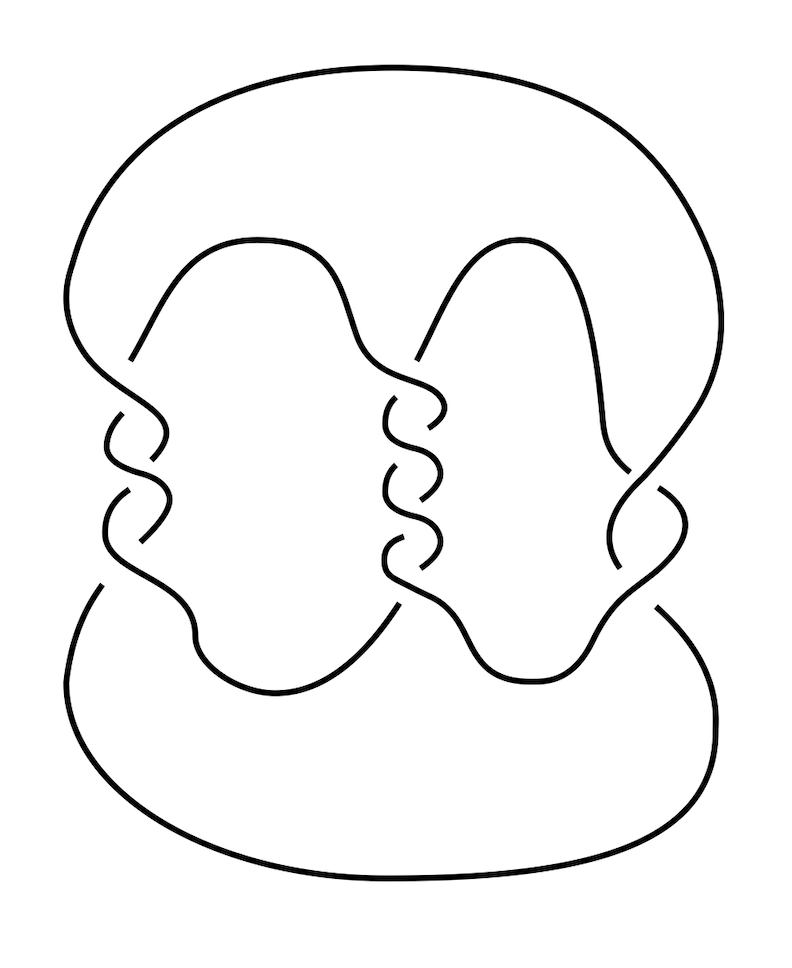
\includegraphics [height=4cm]{augmentation1}&
  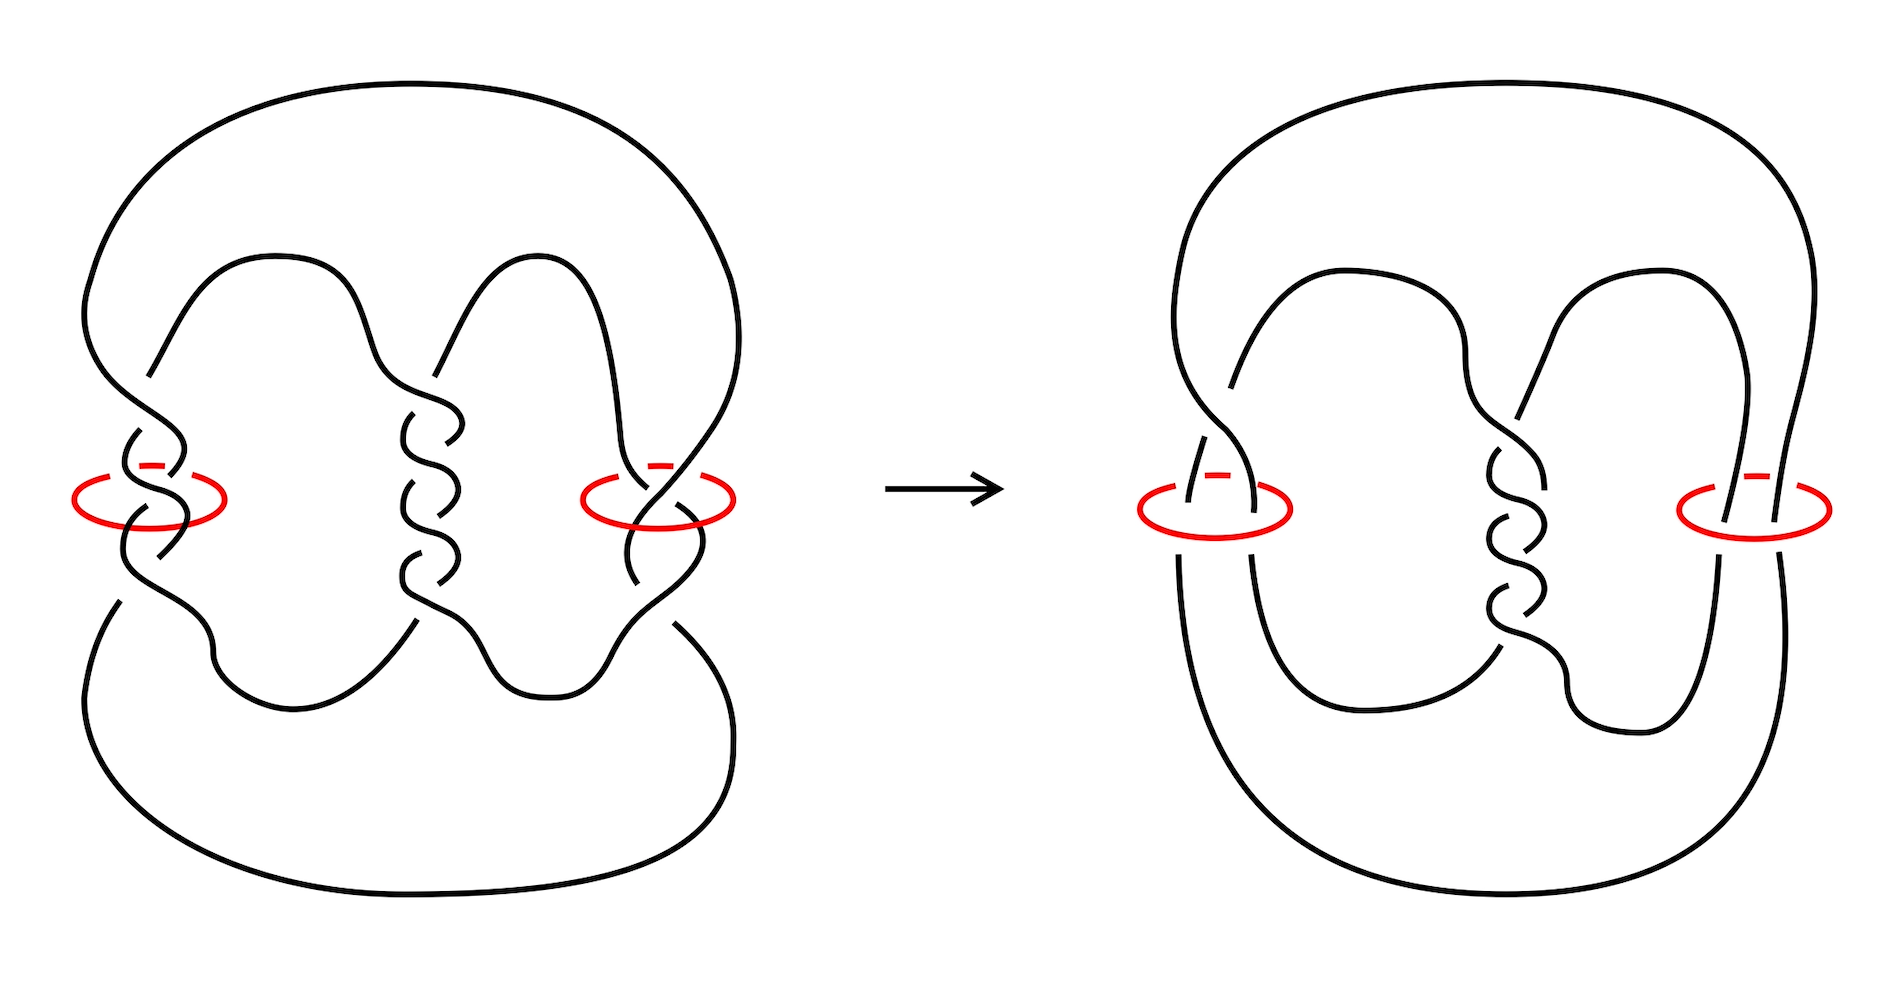
\includegraphics [height=4cm]{augmentation2}\\
  (a)&(b)
  \end{tabular}
 \caption{The left shows a pretzel knot before augmentation and the right shows after augmentation}
 \label{fig:augmentationS3}
 \end{figure}
 
 
 %%%%%%%%%%%%%%%%%%%%%%%%%%%%%%%%%%%%%%%%%%%%%%%%%%%%%%%% 
\section{Augmented Links}
 Champanerkar, Kofman and Purcell have studied alternating links in the thickened torus. They define a link in the thickened torus as a quotient of a biperiodic alternating link as follows,
 
\begin{define}\cite{CKP2} \label{def:biperiodiclink}
 A \emph{biperiodic alternating link} $\mathcal{L}$ is an infinite link which has a projection onto $\R^2$ which is invariant under an action of a two dimensional lattice $\Lambda$ by translations, such that $L=\mathcal{L}/\Lambda$ is an alternating link in $T^2 \times I$, where $I = (-1,1)$, with the projection on $T^2 \times \{0\}$. We call $L$ a link diagram in $T^2 \times I$.   
\end{define}

\begin{remark}
Since $T^2 \times I \cong \Sp^3 - H$, where $H$ is a Hopf link. The complement $T^2 \times I- L = \Sp^3 - (L \cup H)$.
\end{remark}

Champanerkar, Kofman and Purcell \cite{CKP2} extended the definition of prime links in $\Sp^3$ for links in $T^2 \times I$ called weakly prime. 

 \begin{define} \label{def:weaklyprime}
A diagram of a link $L$ is weakly prime if whenever a disk is embedded in the diagram surface meets the diagram transversely in exactly two edges, then the disk contains a simple edge of the diagram and no crossings.
\end{define}


\begin{define}
A \emph{twist region} in a link diagram $L=\mathcal{L}/\Lambda$ in $T^2 \times I$, is the quotient of a twist region in the biperiodic link $\mathcal{L}$. %a string of bigons, or a single crossing in the diagram on the universal cover of $T^2 \times I$ is called a . 
A biperiodic link $\mathcal{L}$ is called \emph{twist-reduced} if for any simple closed curve on the plane that intersects $\mathcal{L}$ transversely in four points, with two points adjacent to one crossing and the other two points adjacent to another crossing, the simple closed
curve bounds a subdiagram consisting of a (possibly empty) collection of bigons
strung end to end between these crossings. We say $L$ is \emph{twist-reduced} if it is the quotient of a twist-reduced biperiodic link. 
\end{define}

Now we can define augmentation for a link in $T^2 \times I$ the same way we define augmentation for links in $\Sp^3$. For a link in $T^2 \times I$, the crossing circles are added to the diagram projected onto $T^2 \times \{0\}$. Let $L$ be a twist reduced diagram in $T^2 \times I$, we define {\it augmentation} as a process in which an unknotted circle component is added to one or more twist regions of $L$. See Figure \ref{fig:Augmentations}


 \begin{figure}
 \centering
 \begin{tabular}{cccc}
 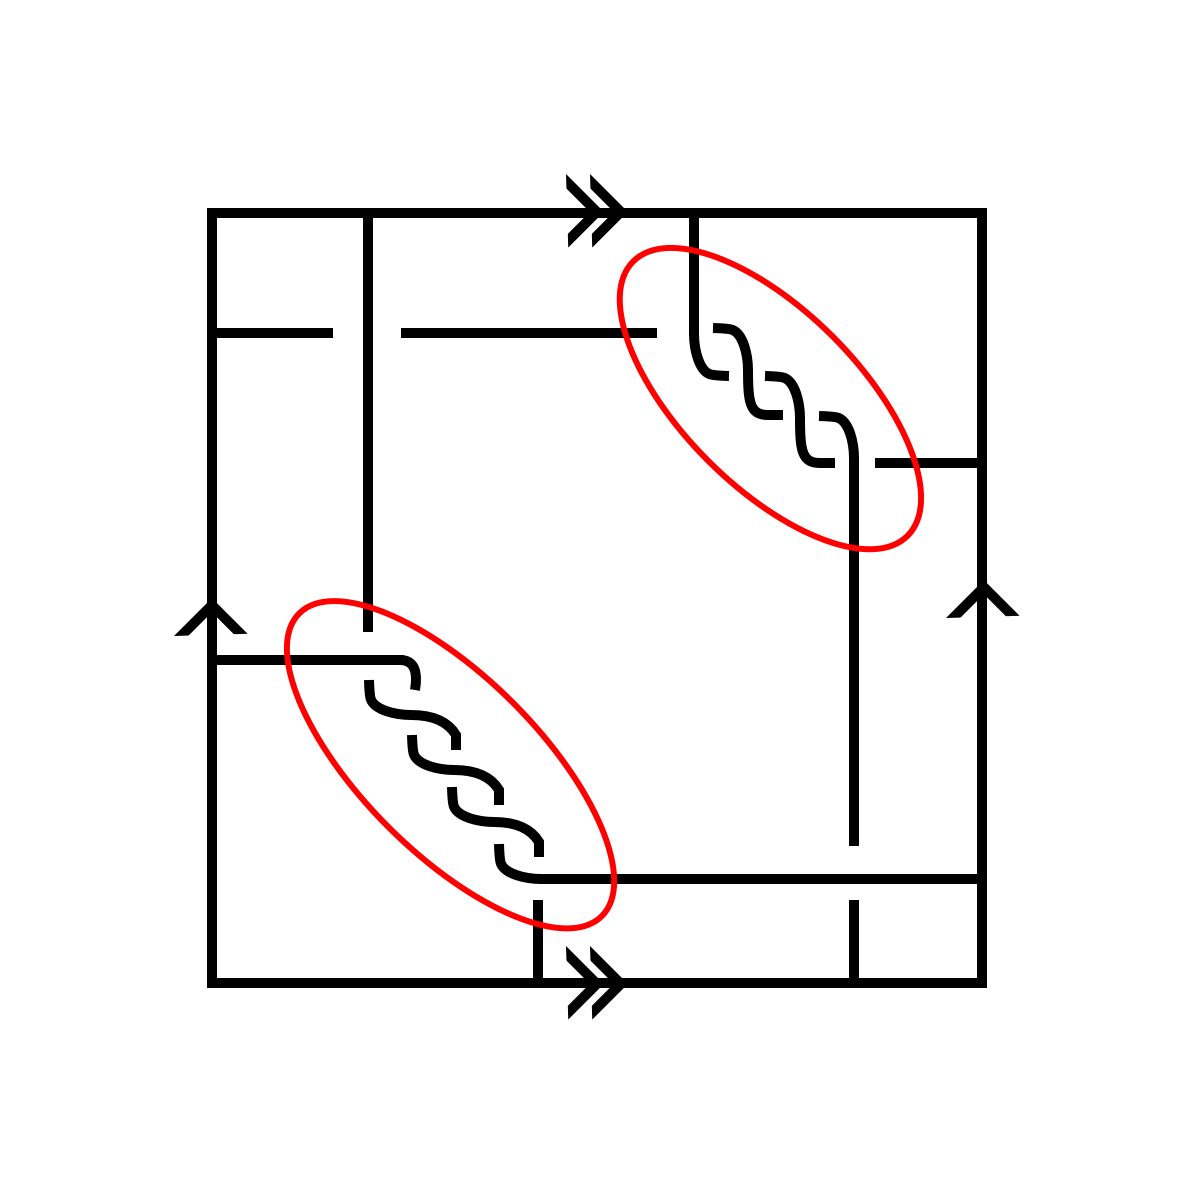
\includegraphics [width=3cm]{fig1}&
 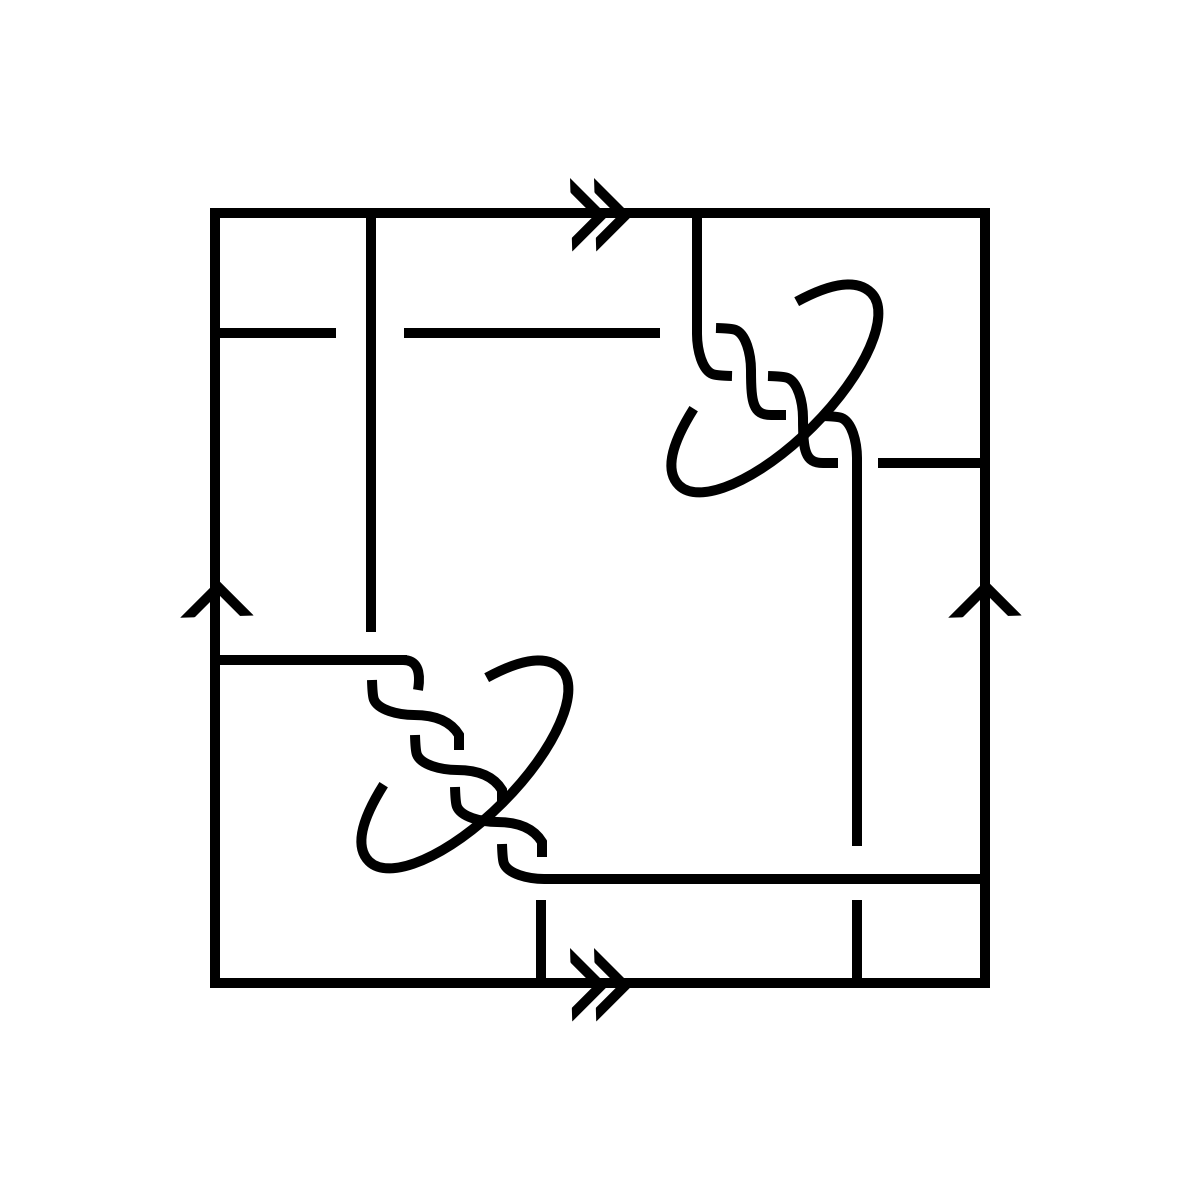
\includegraphics  [width=3cm]{twist-augment}&
  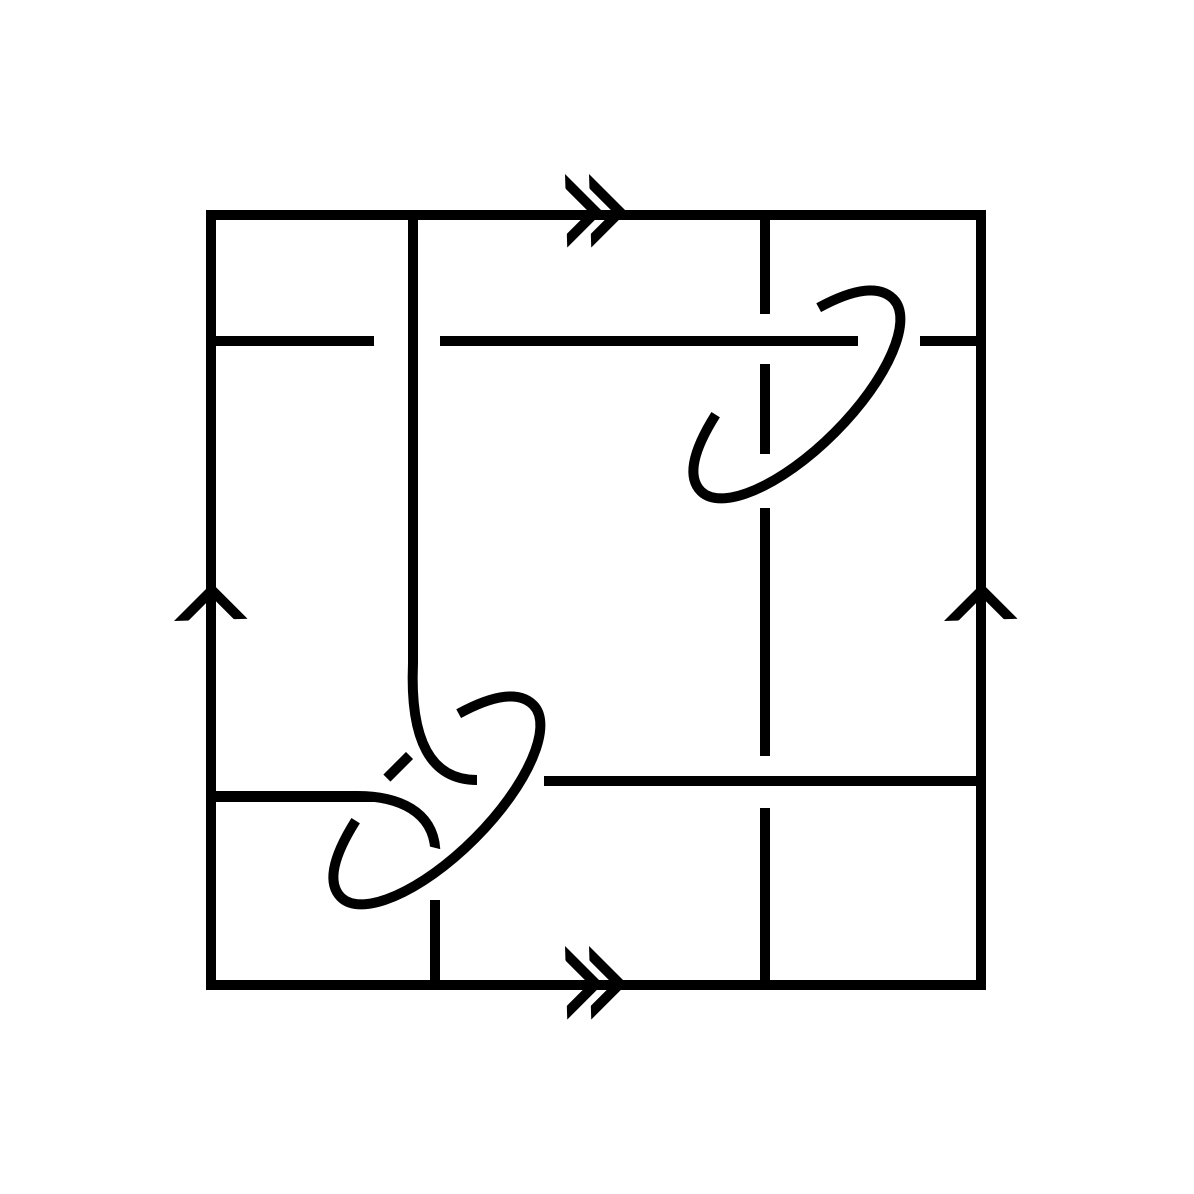
\includegraphics [width=3cm]{fig-2}\\
 % 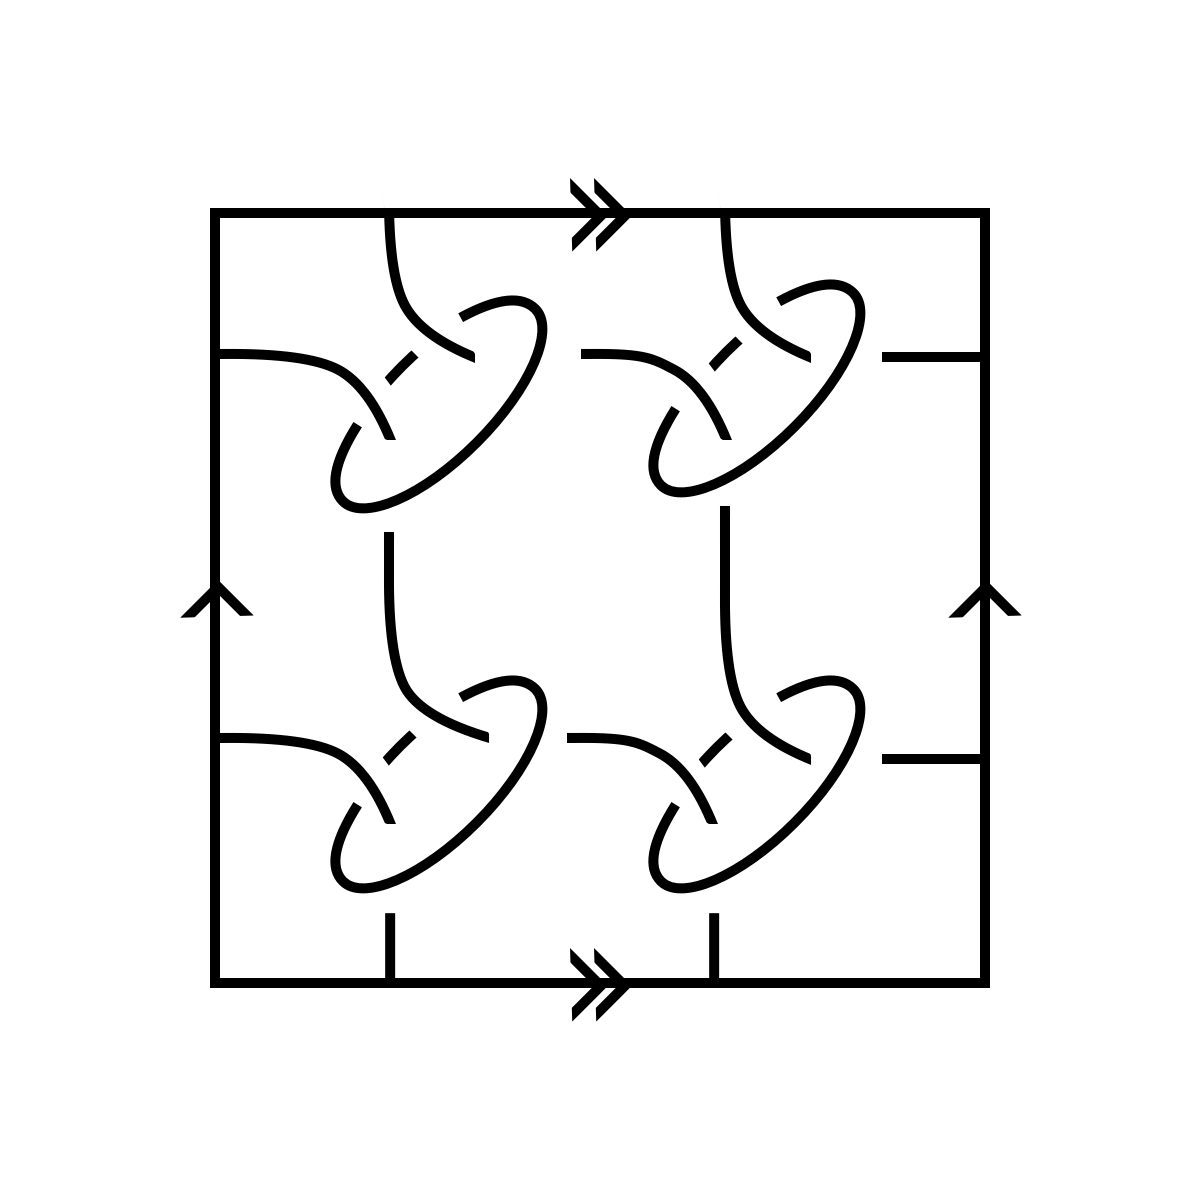
\includegraphics [width=3cm]{fal}\\
  A&B&C
  \end{tabular}
 \caption{A: The top right has an odd number of twists while the bottom left has an even number of twists. B: The picture of the link on the right after augmentation twist regions circled in red. C: The link with the twists removed.}
 \label{fig:Augmentations}
 \end{figure}
%%%%%%%%%%%%%%%%%%%%%%%%%%%%%%%%%%%%%%%%%%%%%%%%%%%% 

\subsection{Torihedral Decomposition of Augmented Alternating Links in Thickened Torus}


We show a method of decomposing an augmented link in the thickened torus into two isomorphic torihedra. The idea is to combine methods of Menasco \cite{Menasco} and the use of crossing edges between each crossing of our link and Lackenby's ``cut-slice-flatten" method \cite{lackenby} on the augmentation sites.   


\begin{define}\cite{CKP2} \label{def:torihedron}
 A \emph{torihedron} is a cone on the torus, i.e. $T^2 \times [0,1]/(T^2 \times \{1\})$, with a cellular graph $G$ on $T^2 \times \{0\}$. An \emph{ideal torihedron} is a torihedron with the vertices of $G$ and the vertex $T^2 \times \{1\}$ removed. Hence, an ideal torihedron is homeomorphic to $T^2 \times [0,1)$ with a finite set of points (ideal vertices) removed from $T^2 \times \{0\}$ 
\end{define}

\begin{prop}\label{thm:torihedraldecomposition}
Let $L$ be an augmented link in $T^2 \times I$. Let $G(L)$ be a diagram of the link on $T^2 \times \{0\}$. There is a decomposition of the complement, $(T^2 \times I) - L$ into two isomorphic ideal torihedra.
\end{prop}

\textit{Proof}. We will begin by assuming that there are no half twists and then arrange the link diagram of $L$ in the following way: first place the added circle components (augmentation) perpendicular to the projection plane, $T^2 \times \{0\}$ leaving the remaining part of the link parallel to the projection plane. 
We now place a crossing edge on each crossing of the link so that for each crossing edge, one end of the edge lies on a bottom strand while the other end lies on a top strand as in Figure \ref{fig:crossingArc} left.

\begin{figure}
 \centering
 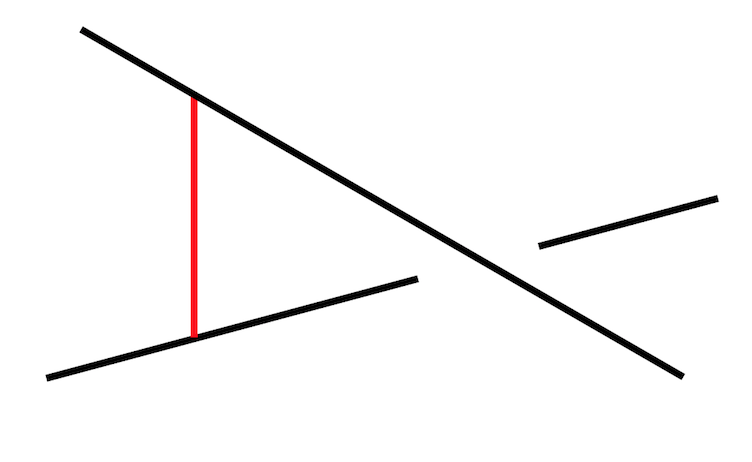
\includegraphics[width=4cm]{crossingArc}
  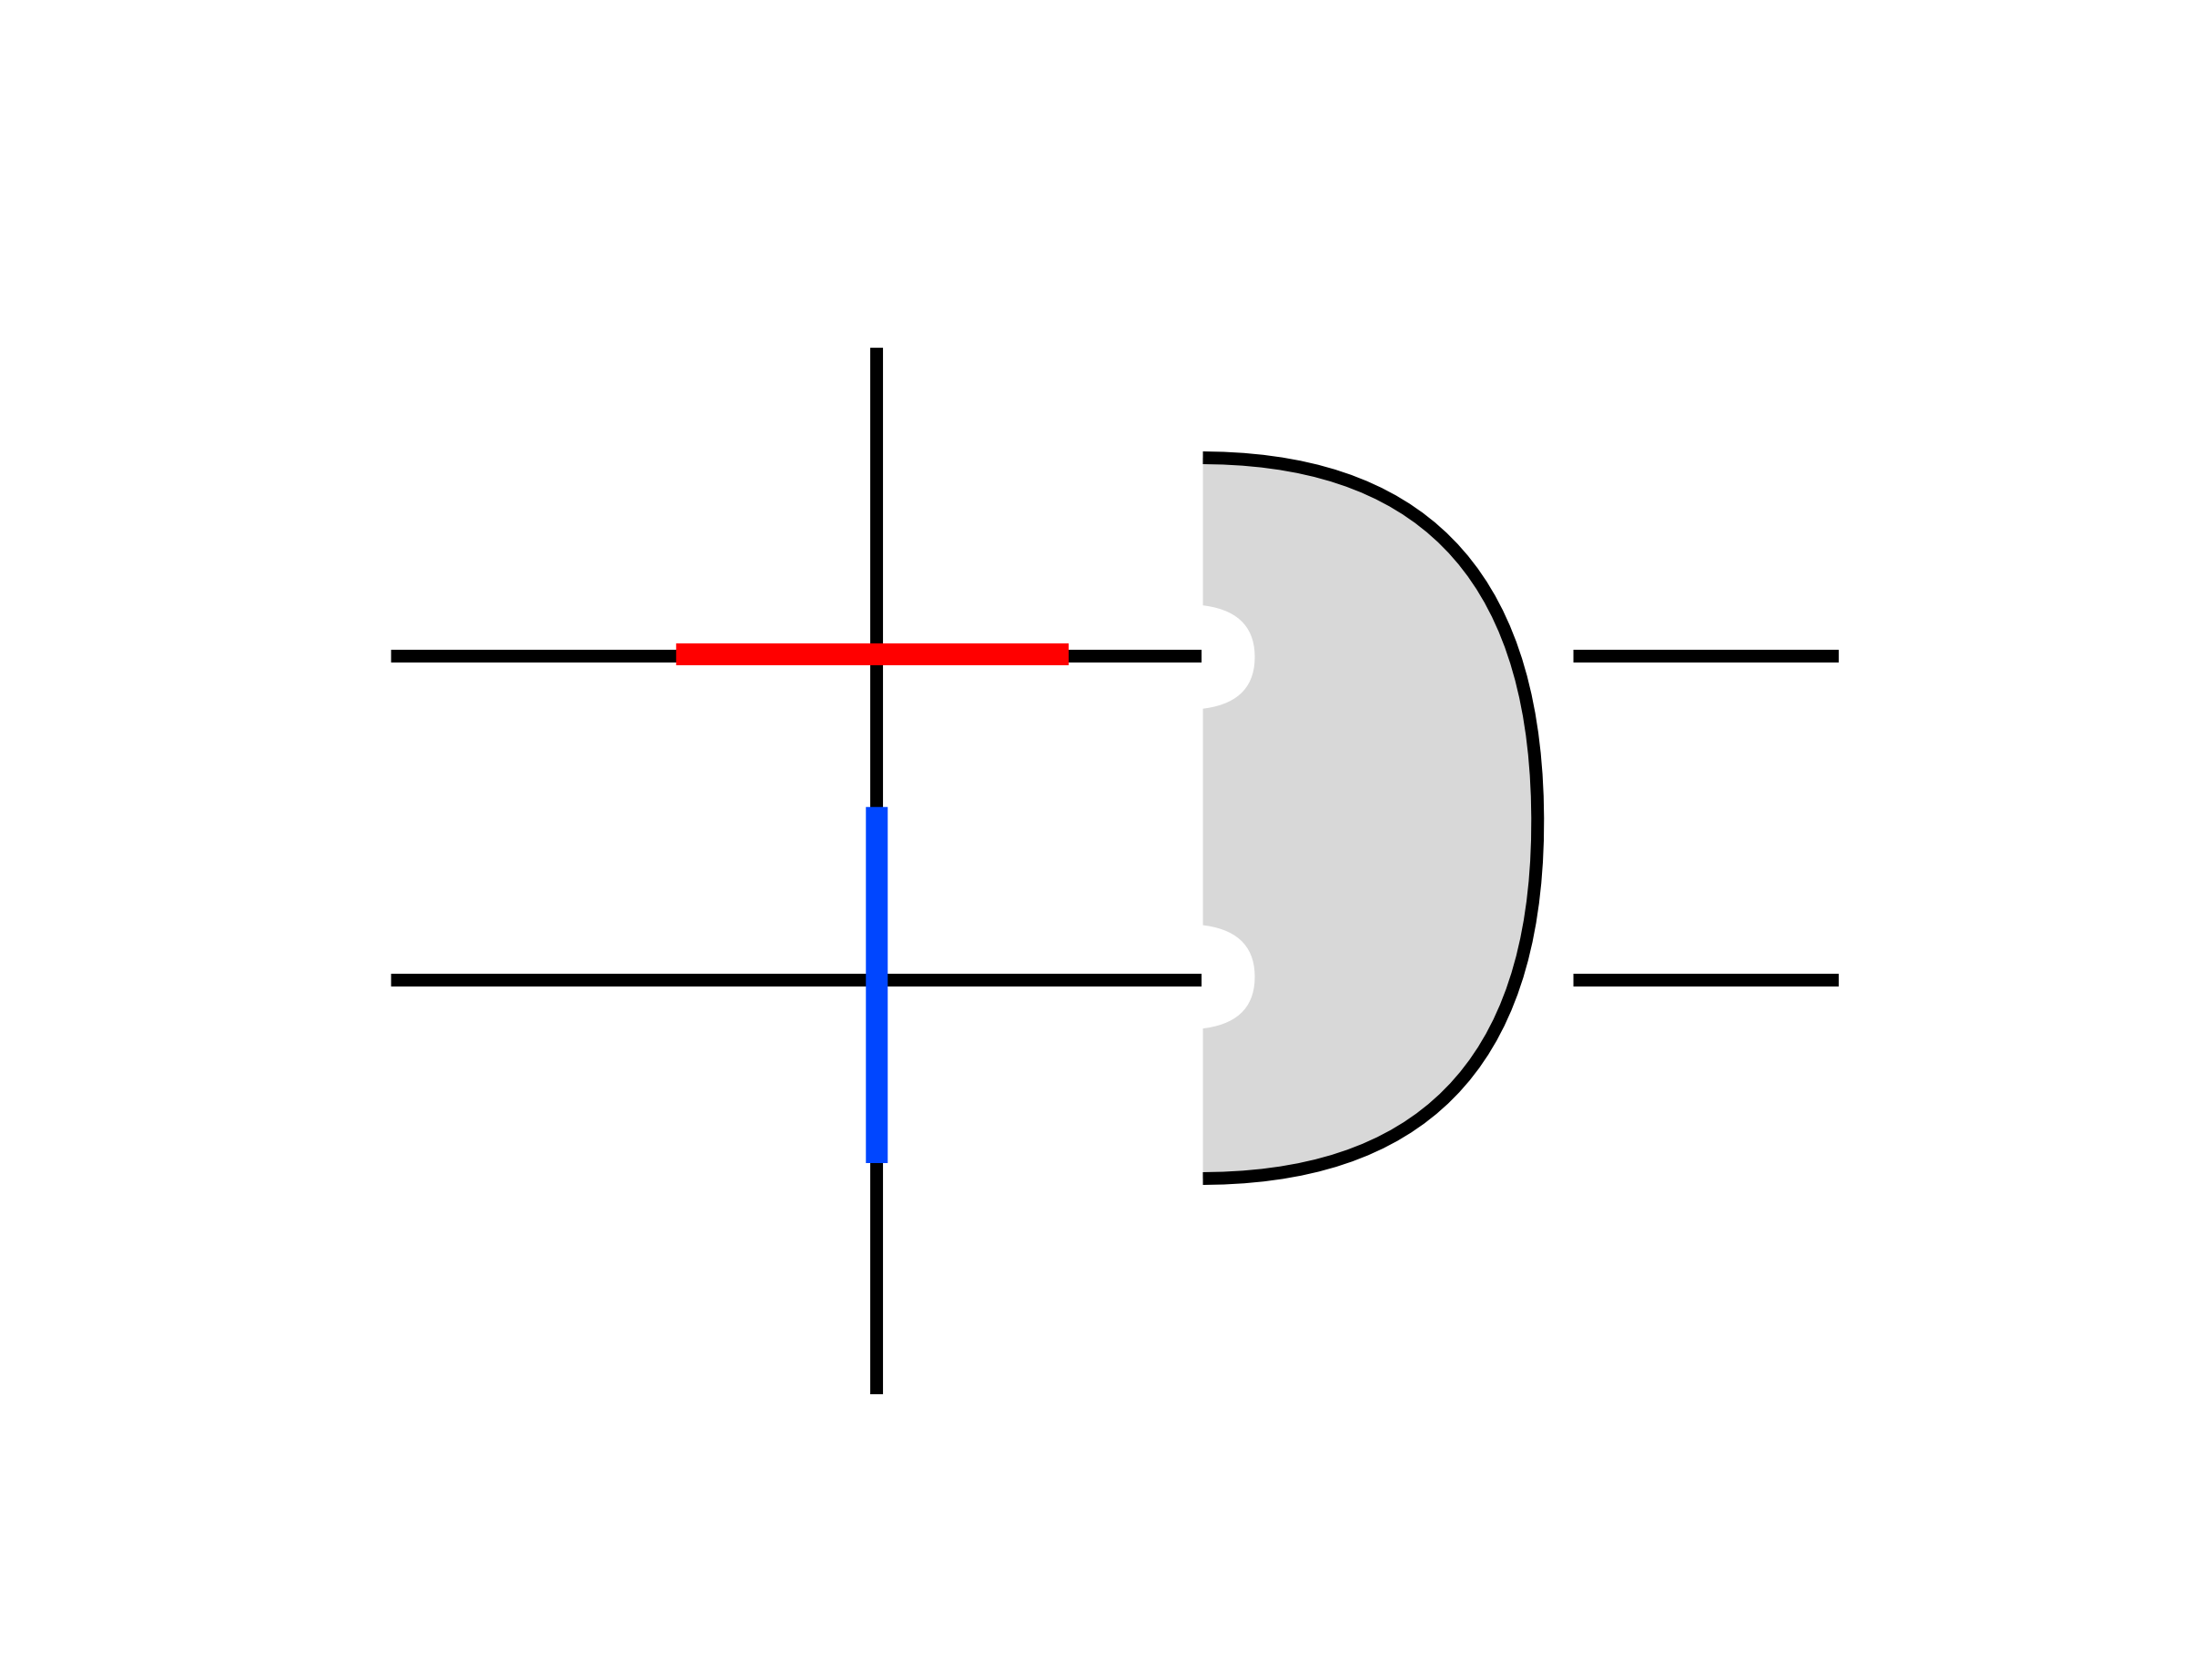
\includegraphics[width=5cm]{crossingPush}
 \caption{Left: The black strands are part of the link and the red strand is the crossing edge. Right: The blue and red edges represent the split crossing edges and the shaded half disk is bounded by the crossing circle}
 \label{fig:crossingArc}
 \end{figure}

\indent We view the link from the point at infinity from the top. We will push the top strand to the bottom strand, splitting the crossing edge into two identical edges as in Figure \ref{fig:crossingArc} right. We push the link components to infinity and stretch the crossing edge so that we have flattened the link onto $T^2 \times \{0\}$ except for the crossing circles which will remain perpendicular to the projection plane. 
 
\indent Now place a disk on each crossing circle, so that the disk bounded by the crossing circle. We can then cut $T^2 \times I$ along $T^2 \times \{0\}$ and focus on the top half, $T^2 \times [0,1)$. We will follow the same method on the bottom half to obtain the second identical torihedron. The disk we place on each crossing circle is now cut in half. This half disk is now bounded by the projection plane and the semi-cricle arc of the crossing circle. We push down on the crossing circle and split the disk into two identical disks. We then push the arc of each crossing circle to infinity, collapsing them to ideal vertices. We obtain two triangular faces which represent the disk which look like a bow-tie as in Figure \ref{fig:falGluings}. 

\begin{figure}
 \centering
 \begin{tabular}{cc}
 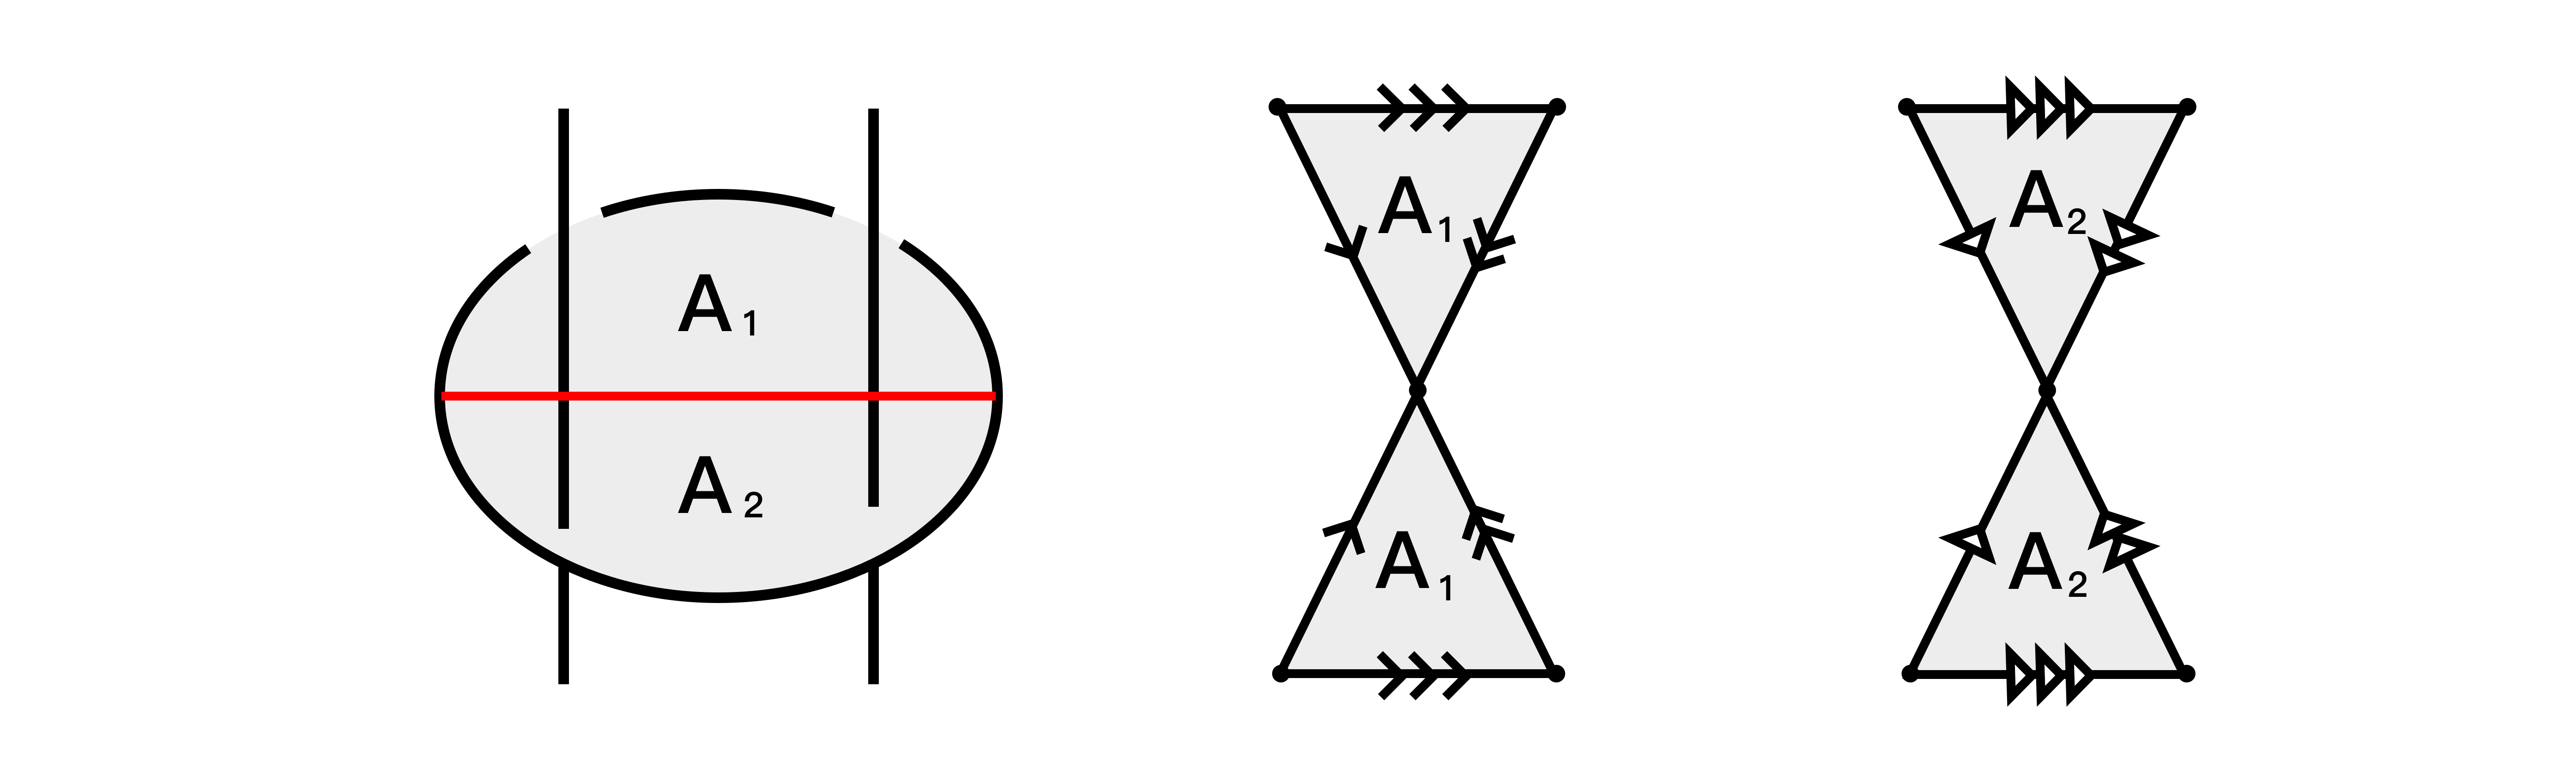
\includegraphics [width=8cm]{falGluing1}&
 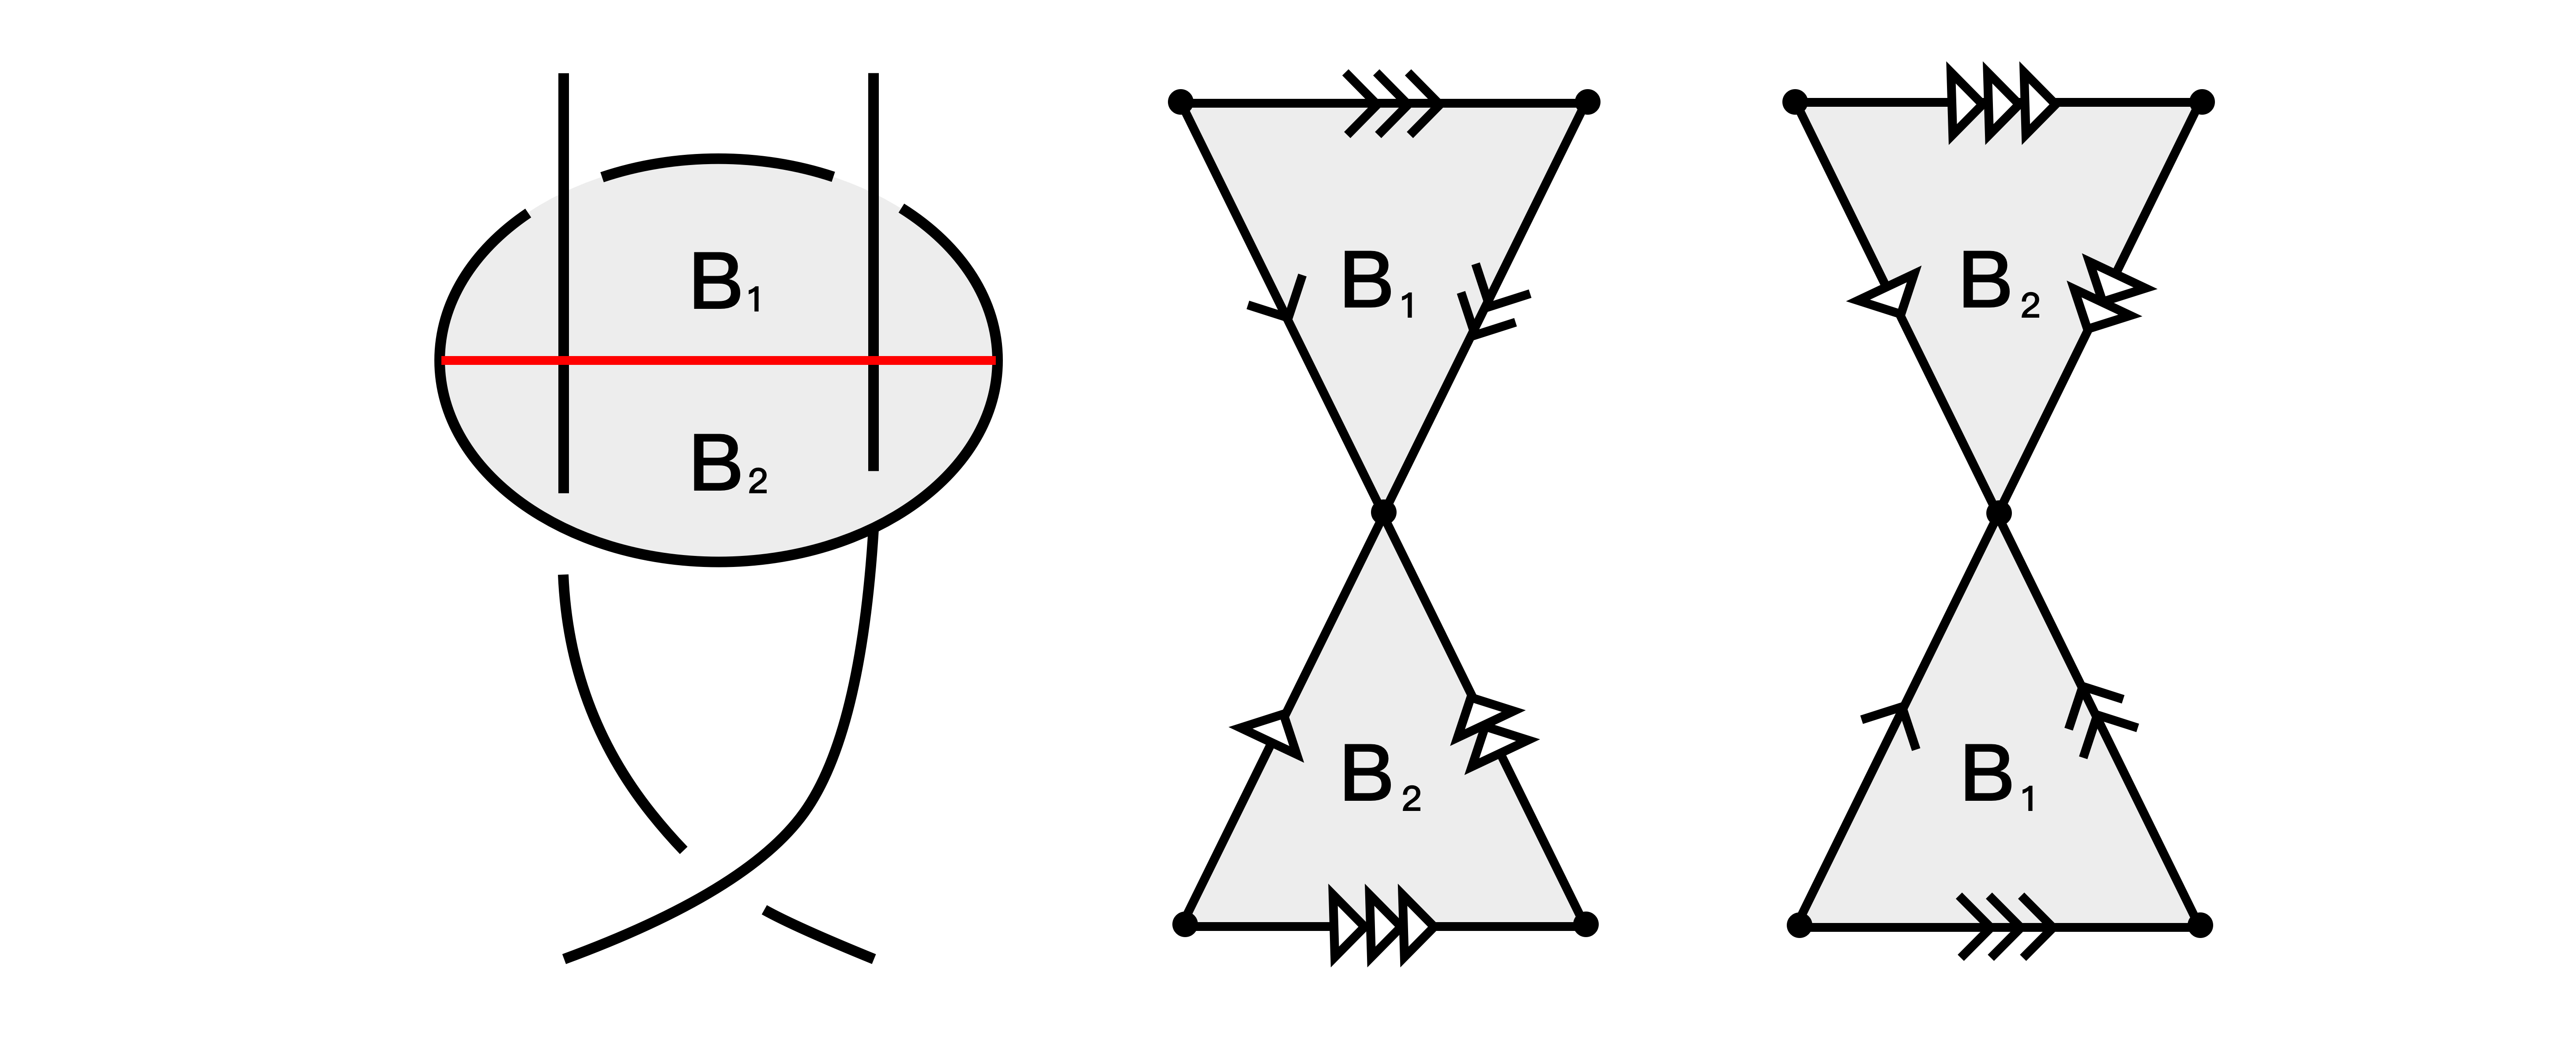
\includegraphics [width=7cm]{falGluing2}\\
 (a)&(b)
 \end{tabular}
 \caption{The first pictures shows gluing without half-twists the second shows gluing with half-twists}
 \label{fig:falGluings}
 \end{figure}

\indent We repeat the steps for the bottom half of $T^2 \times I$, $T^2 \times [-1,0)$. Then we get two isomorphic torihedra. The graph of each will come from crossing edges and, edges of the disk. Now, if there are half twists we will decompose the complement of the link the same way as if there are no half twists and we will identify the two bow-ties as in Figure \ref{fig:falGluings}. Finally we obtain the complement of the link by gluing the two torihedra with the gluing information given by identifying crossing edges and triangles of the bow-tie. We glue the faces of the torihedra which do not correspond to a bow-tie with a $\pi/n$ twist where $n$ is the number of sides of each face as in Figure \ref{fig:top-bottom} clockwise or counterclockwise. \qed

%%%%%%%%%%%%%%%%%%%%%%%%%%%%
The following figures is an example which decomposes the link (C) of Figure \ref{fig:Augmentations}.
 \begin{figure}[h]
 \centering
 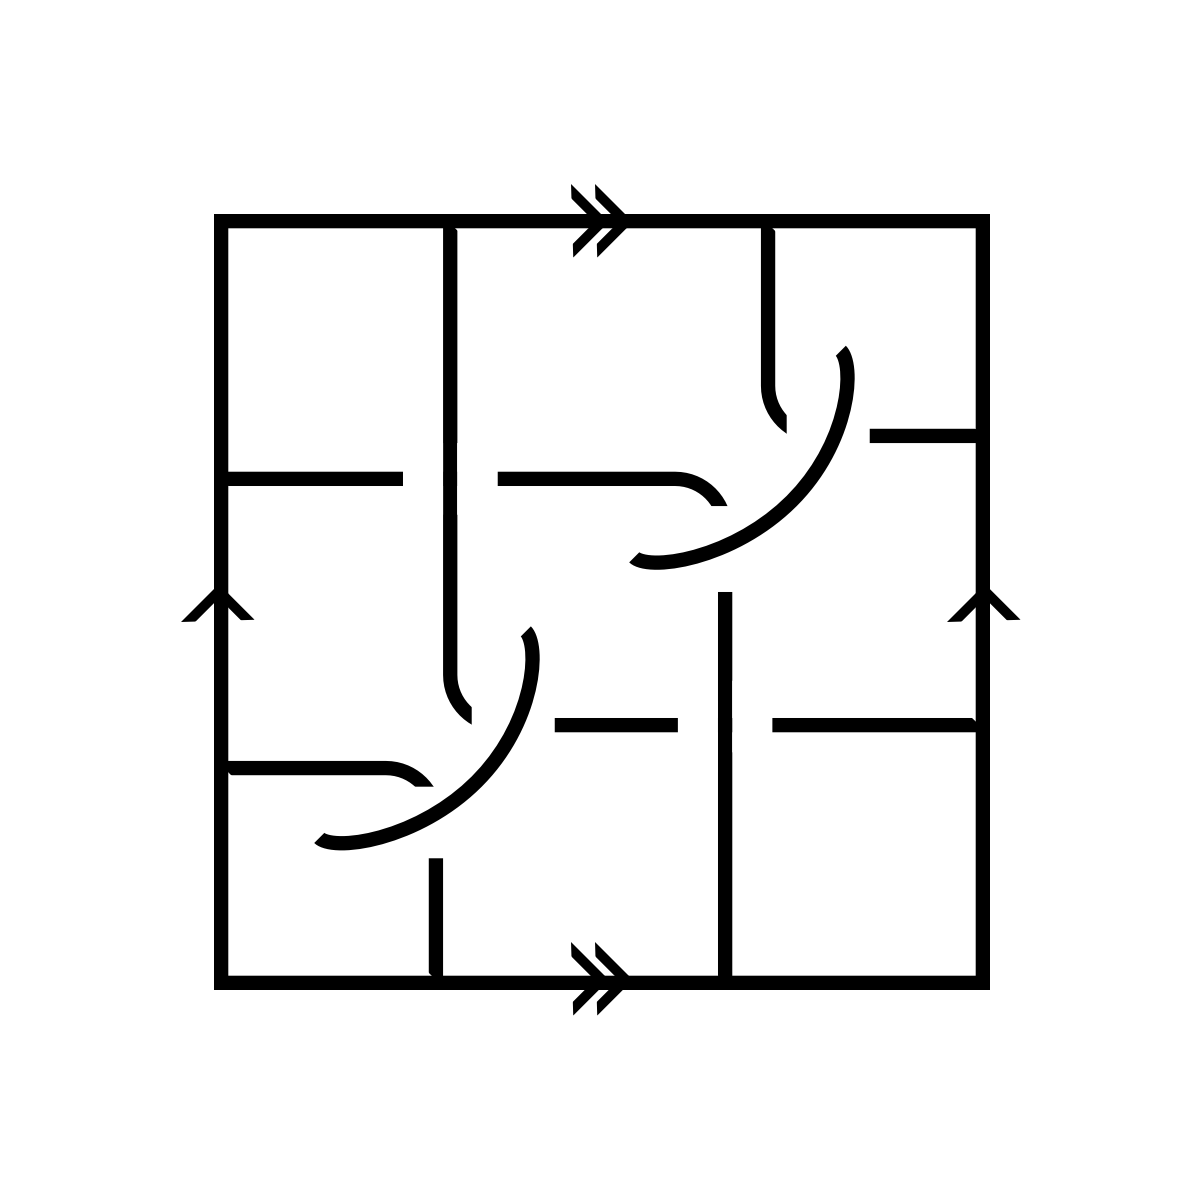
\includegraphics [height=3cm]{fig-3}
 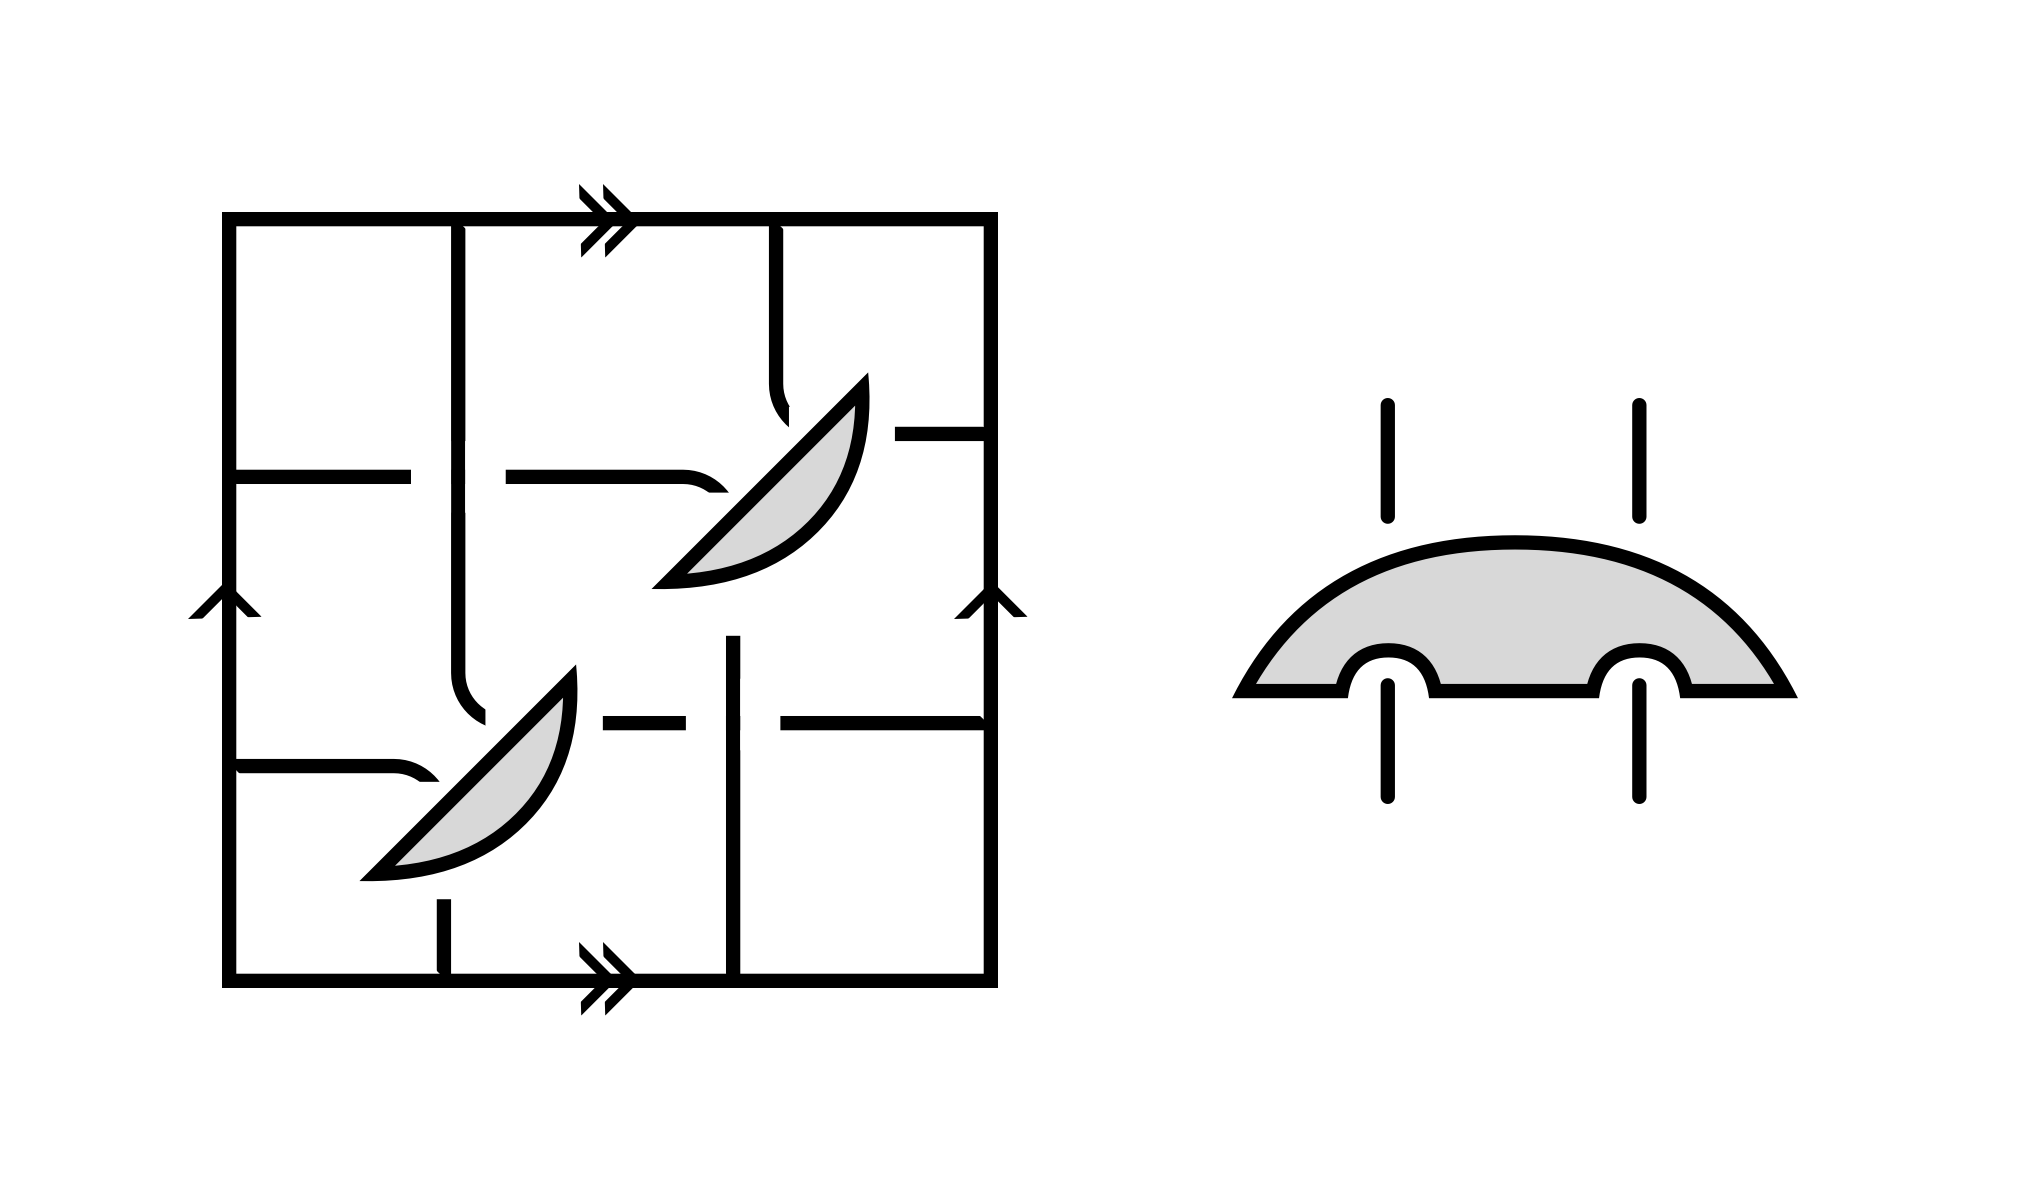
\includegraphics [height=3cm]{fig-4}
 \caption{Each crossing circle bounds a disk}
 \end{figure}
 
 \vspace*{-0.5cm}
  \begin{figure}[h]
\centering
 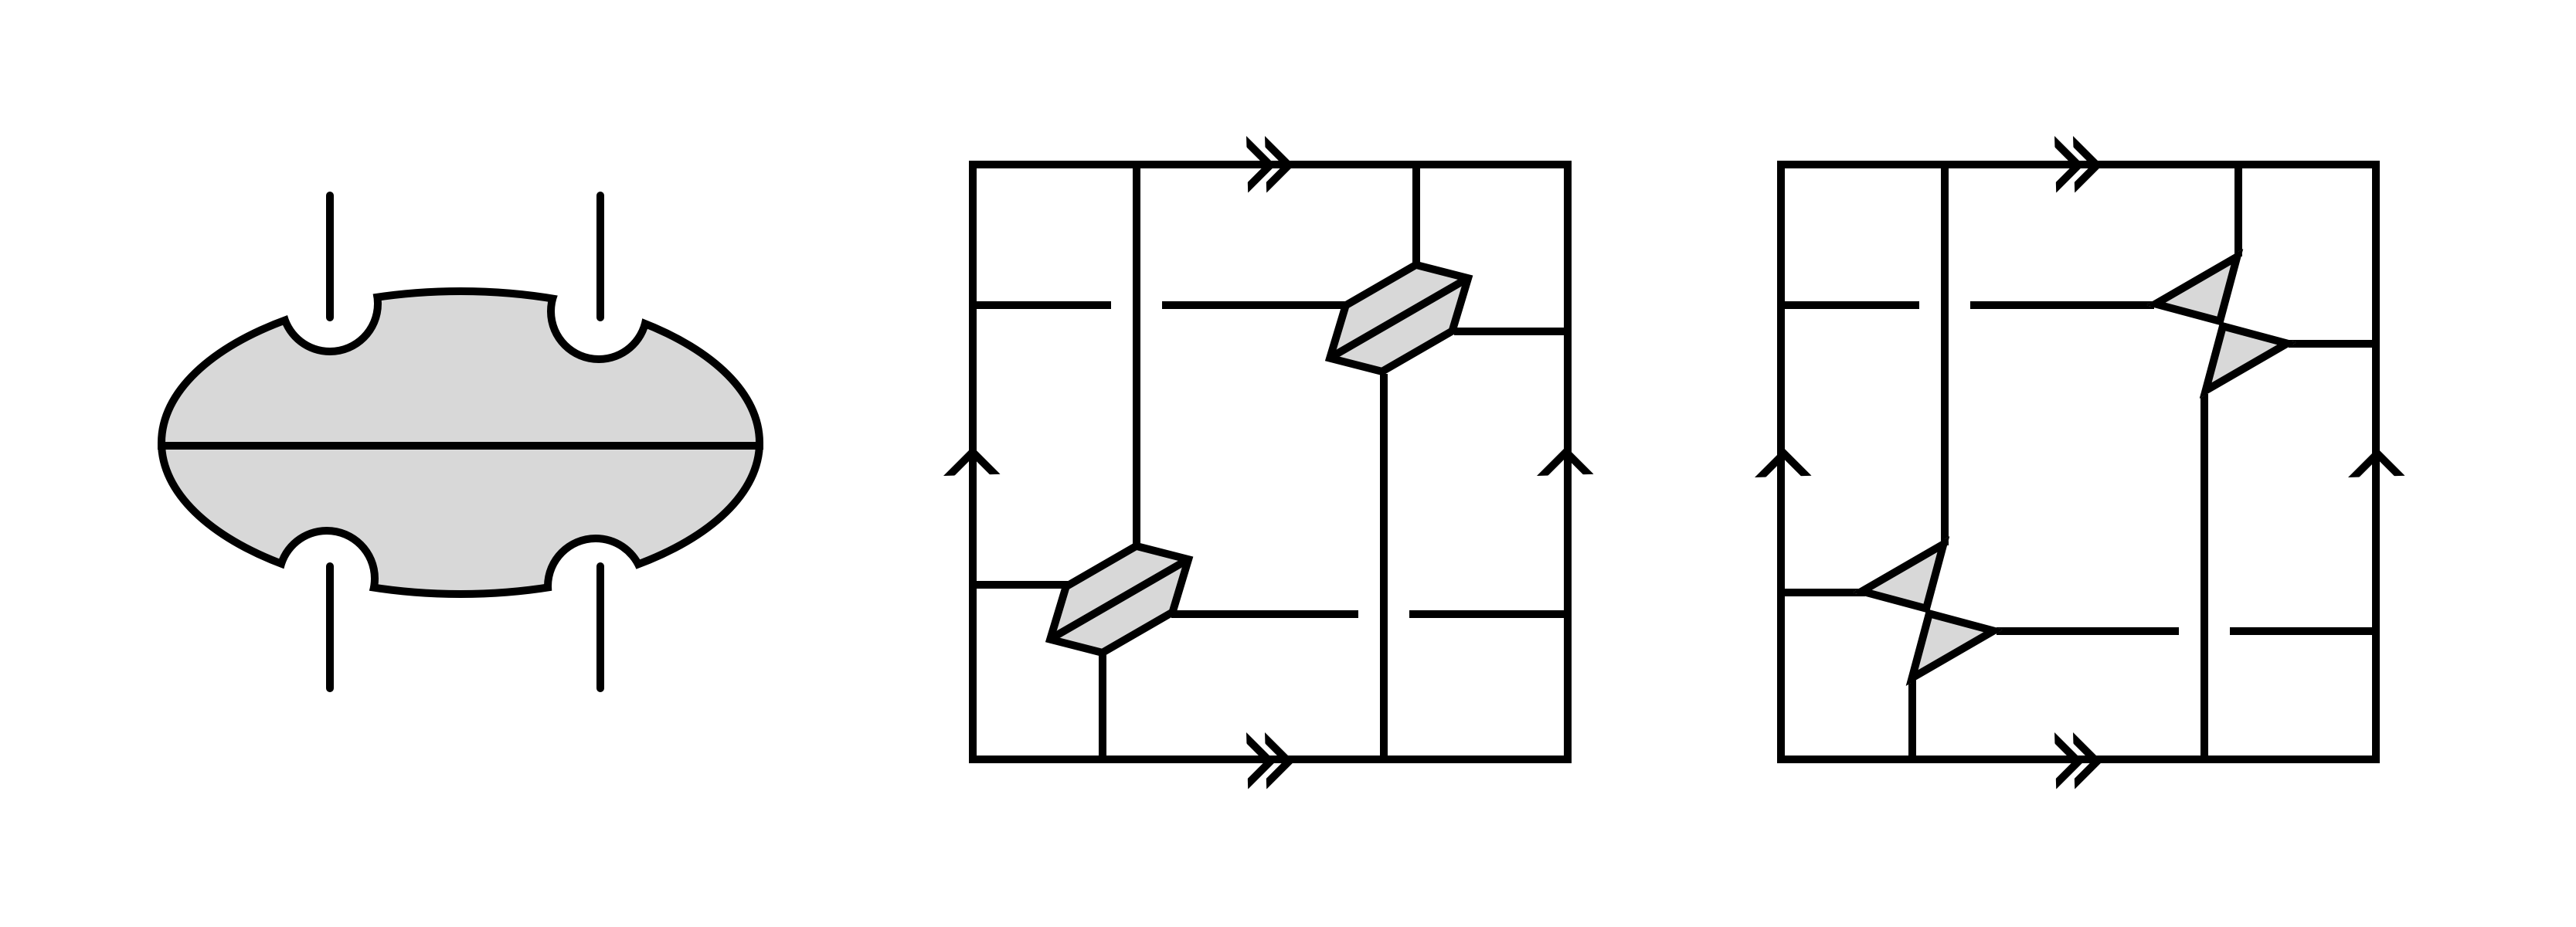
\includegraphics [height=3cm]{fig-5}
 \caption{We split the disk and collapse the arc of each crossing circle to ideal vertices}
 \end{figure}
 
  \vspace*{-0.5cm}
  \begin{figure}[h]
 \centering
 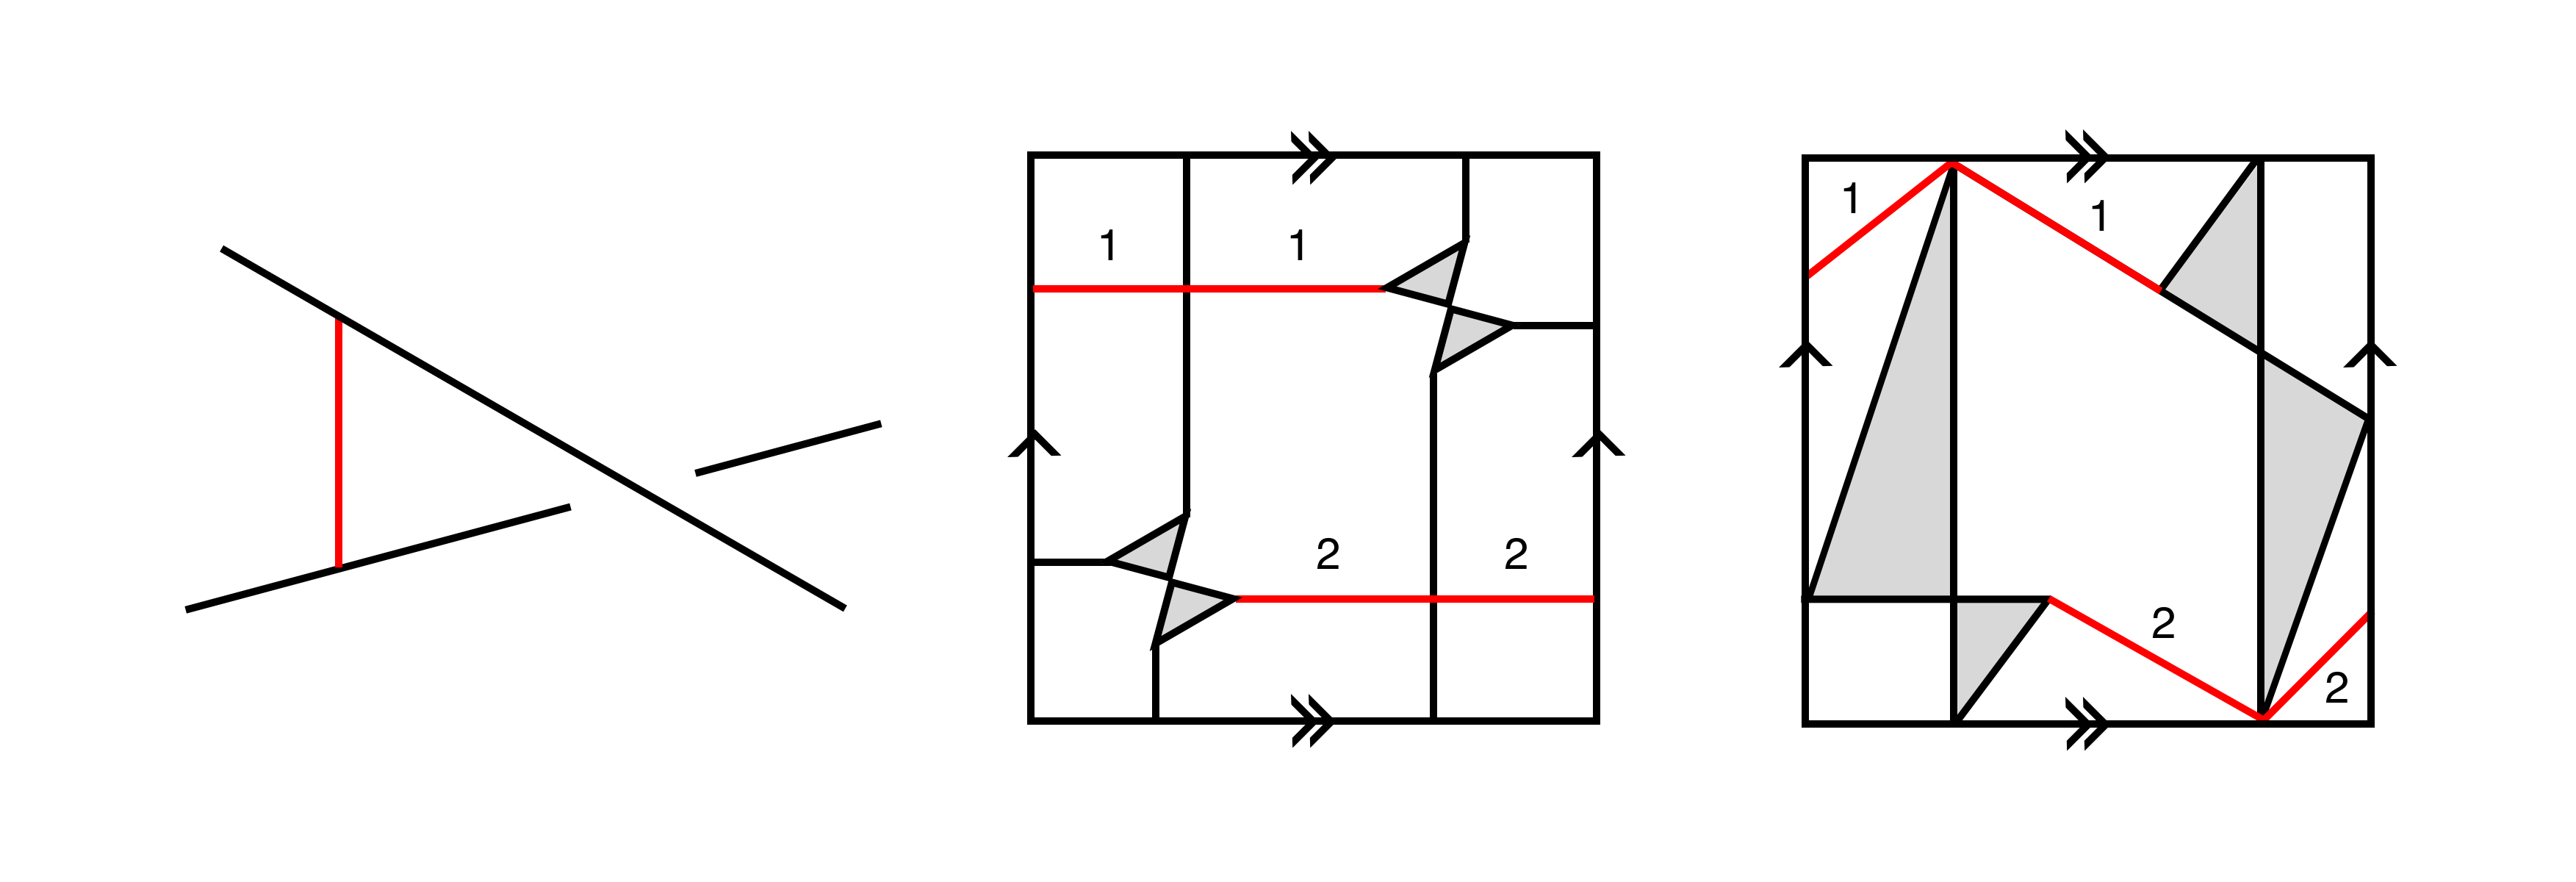
\includegraphics [height=3cm]{fig-6}
 \caption{Left: The crossing arc is the edge in red. Middle: Picture of splitting the crossing edge. Right: The link component is pushed off to infinity.}
 \end{figure}

 \vspace*{-0.5cm}
 \begin{figure}[h]
 \centering
 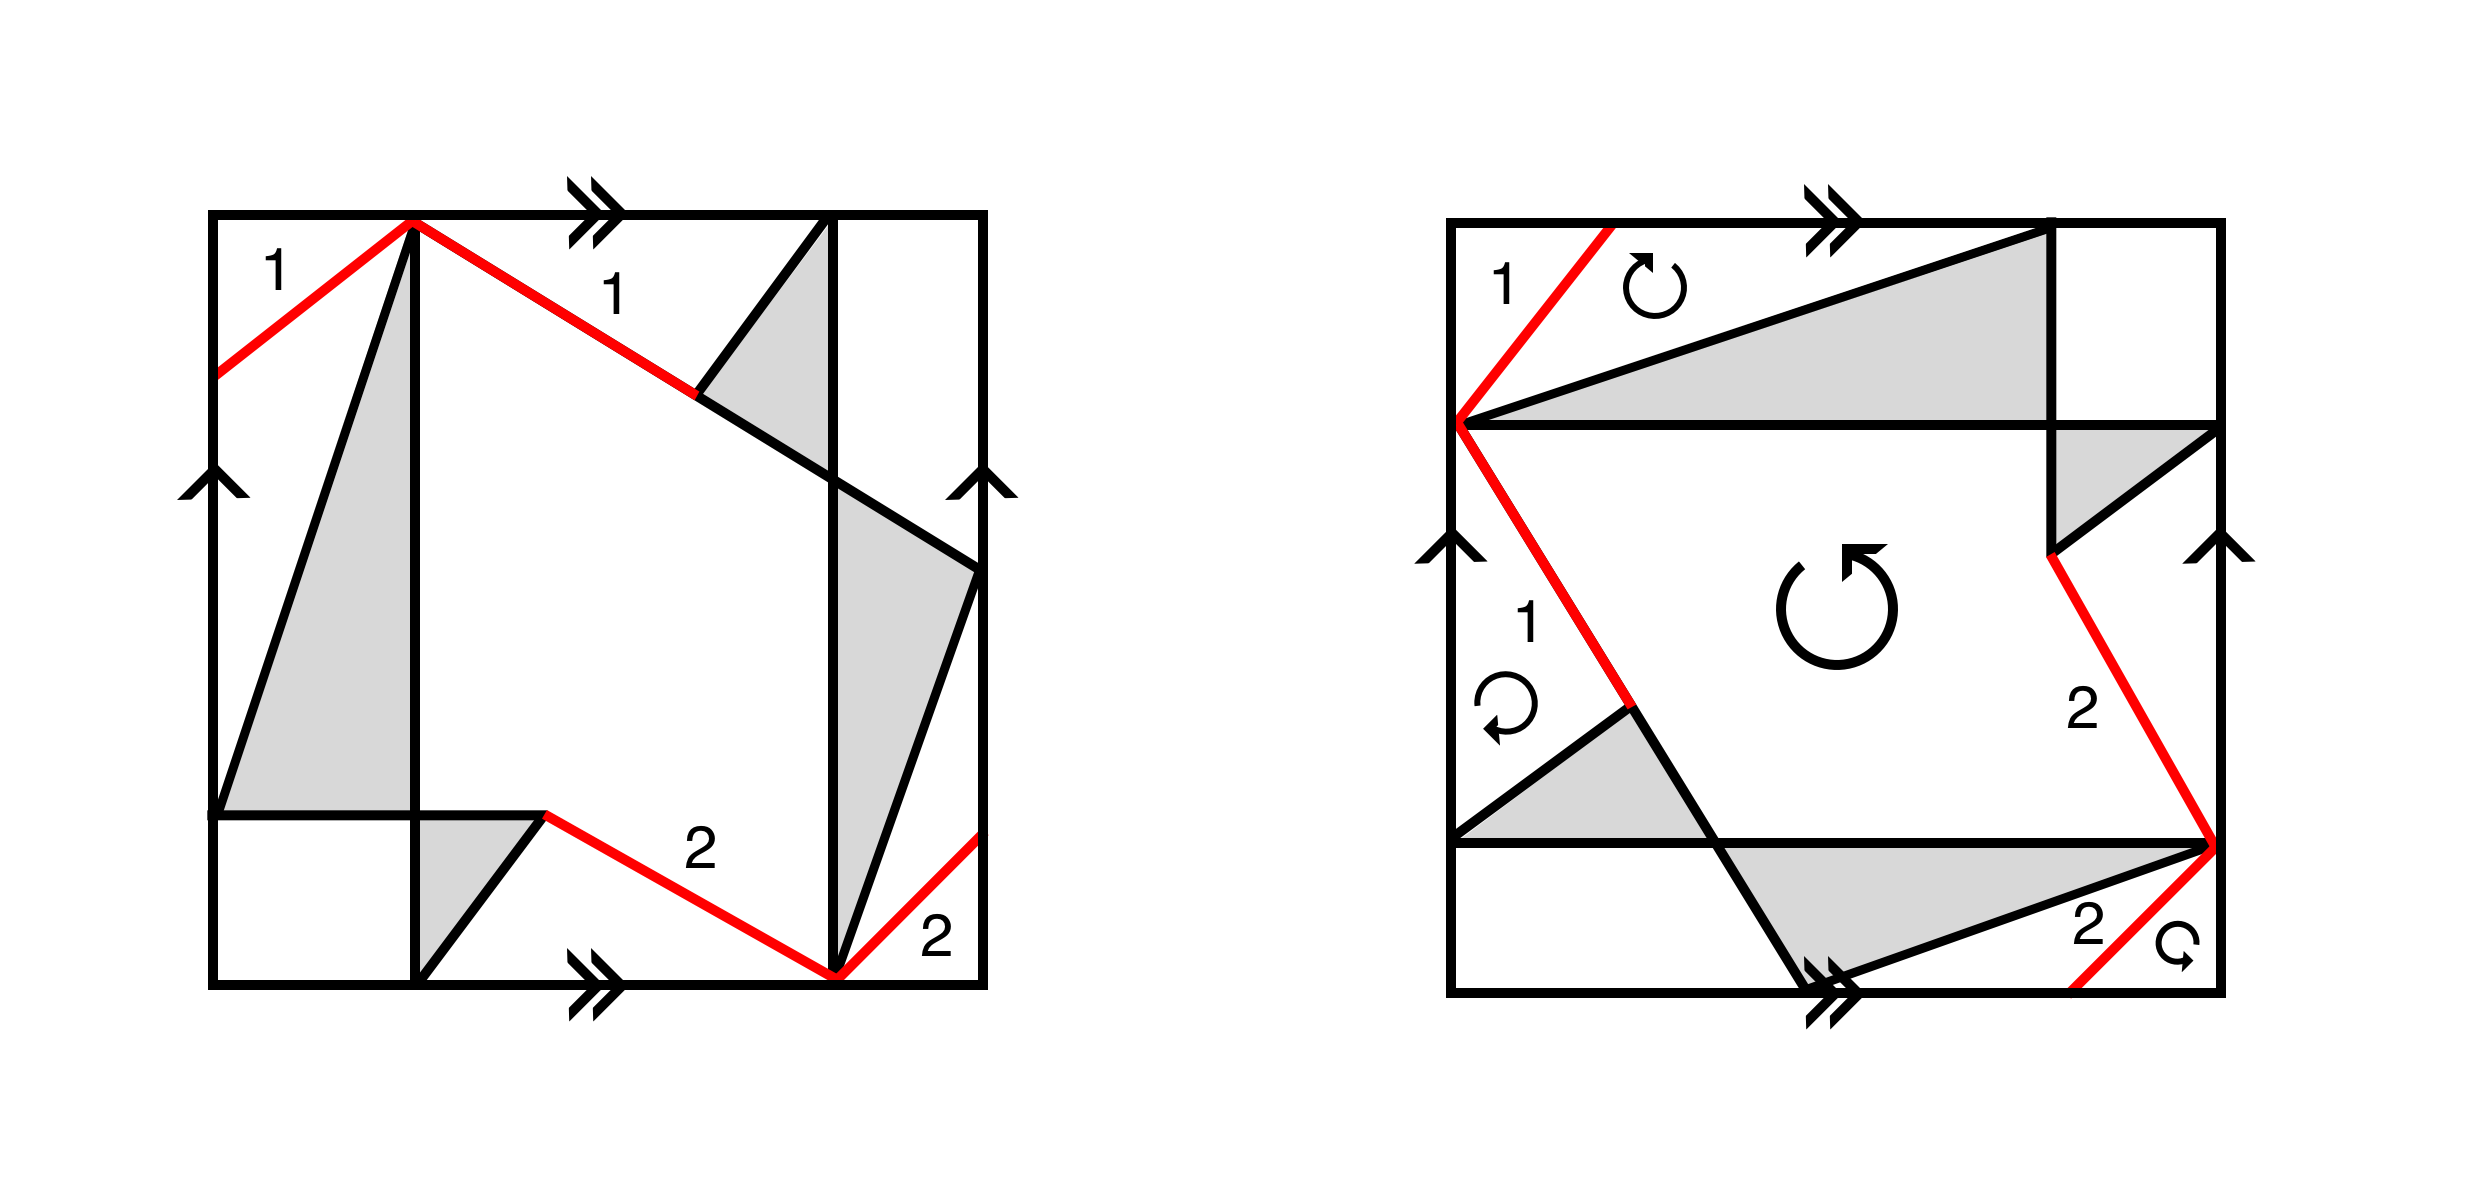
\includegraphics [height=3cm]{top-bottom}
 \caption{Left: The top torihedron. Right: The bottom torihdron with rotation for face gluing.}
 \label{fig:top-bottom}
 \end{figure}

\begin{remark}\label{cor:triangulation}
The faces of one torihedron which do not correspond to a bow-tie glue to a corresponding face of the second torihedron to form bipyramids. One can add stellating edges, edges which have vertices corresponding to the different components of the Hopf link that cuts through the center of the face to decompose the bipyramids into tetrahedra. This process is called {\it stellation}. Stellating all the bipyramids of the decomposition obtained from Proposition \ref{thm:torihedraldecomposition} we obtained a triangulation of the complement of $L$ which is made up of {\it horizontal} edges (edges from the graph of the torihedra), {\it vertical} edges (edges from coning vertices of the the graph of the torihedra) and stellating edges. 
\end{remark}

{\it Proof.}  Using the decomposition from Proposition \ref{thm:torihedraldecomposition} we can add a stellation edge whose end points are $T^2 \times \{-1\}$ and $T^2 \times \{1\}$ which cut through faces of $T^2 \times I$ which do not come from the augmentation disks like in \cite{CKP2}. Since each face of the top torihedron gets glued to the bottom torihedron, we obtain bipyramids, and the stellation edge will decompose the bipyramids into tetrahedra. Then the link of the vertex  $T^2 \times \{1\}$ or $T^2 \times \{-1\}$ is the graph of the torihedron $T^2 \times [0,1)$ or $T^2 \times (-1,0]$ respectively. \qed

\section{Hyperbolicity of Augmented Links}

We will use angle structures and a result by Casson-Rivin which shows that if one has angled triangulation manifold is hyperbolic. 

\begin{define}
angle structure
\end{define}

\begin{theorem}\cite{ANGLE STRUCTURE PAPER}
casson-Rivin theorem
\end{theorem}

For a hyperbolic link $K$ in $T^2 \times I$, we produce sufficient conditions on augmentations such that the resulting link obtained from augmenting $K$ is hyperbolic. The idea is to start with a graph from the torihedral decomposition of the link $K$ which will give us a graph on each torihedron with $\pi/2$ edges \cite{CKP}. Then there is corresponding right-angled circle pattern \cite{B-S}. We then consider the augmented link torihedral decomposition from Proposition \ref{} with a corresponding ``degenerate" circle pattern. We then deform this degenerate circle pattern into a ``proper" circle pattern which will give us a polyhedral decomposition with angles of the torihedra in our torihedral decomposition. Which we can further decompose into tetrahedra with angles satisfying conditions of an angle structure. 


\begin{define}
An \emph{angled ideal tetrahedron} is an ideal tetrahedron with an assignment of a dihedral angle
to each edge, such that
\begin{itemize}
\item each dihedral angle is between 0 and $\pi$;
\item for each tetrahedron, opposite edges have equal dihedral angles;
\item the three distinct angles sum to $\pi$.
\end{itemize}
\end{define}


\begin{lemma}
Let $P_n$ be an ideal pyramid whose base is an $n$-gon and suppose,
\begin{itemize}
\item each boundary edge of the original base face is assigned a dihedral angle $\alpha_i$ such that for adjacent edges, $\alpha_i + \alpha_{i+1} < \pi$;
\item we are given a decomposition of the base face into triangles by adding new edges. 
\end{itemize}
One gets an obvious corresponding triangulation of $P_n$, where a new face is added for each new edge. Then there is an assignment of a dihedral angle to each edge of each ideal tetrahedron in this triangulation such that
\begin{itemize}
\item each tetrahedron is an angled ideal tetrahedron;
\item the sum of dihedral angles around each new edge is $\pi$;
\item the dihedral angles of the edges of the original base face are the same as before.
\end{itemize} 
\end{lemma}

{\it Proof.} See Figure \ref{TODO}

\begin{define}
We say an augmentation is \emph{right-augmented} when both strands are (locally) oriented such that they cross the augmentation disk in the same direction, the crossing is positive/ a right-handed half-twist. See Figure \ref{TODO}
We say an augmentation is \emph{left-augmented} if it is not right-augmented.
\end{define}

\begin{define}
Given a face $f$ of the original link diagram the \emph{augmentation sequence} of $f$, denoted $\sigma_f$ is a sequence of symbols $0, L, R$ indexed by vertices of $f$ going counter-clockwise, where, for $v \in \partial f$, the $v$-th element is
\[
\sigma_f^v = 
\begin{cases}
0 \text{ if $v$ is not augmented} \\
L \text{ if $v$ is left-augmented} \\
R \text{ if $v$ is right-augmented}
\end{cases}
\]
\end{define}

\begin{theorem}
Let $K$ be a weakly prime, alternating link with diagram $D$ with no bigons. Let $L$ be a link obtained from augmenting $K$ such that:
\begin{enumerate}
\item there exist no sequence of augmentations so that a Left augmentation is adjacent to a Right augmentation;
\item the sequence of augmentations does not contain a subsequence $0, L, L, 0$ and $0, R, R, 0$.
\end{enumerate}  
Then $L$ is hyperbolic.
\end{theorem}

{\it Proof.}

\bibliographystyle{plain}
\bibliography{references-ak}

\end{document}
